%<dscrpt>Inégalité isopérimétrique pour un polygone.</dscrpt>
Ce problème porte sur \emph{l'inégalité isopérimétrique} reliant l'aire et le périmètre de certaines figures géométriques.\newline
Dans tout le problème, $n$ désigne un entier supérieur ou égal à $3$ et $\omega$ désigne $e^{i\frac{2\pi}{n}}$.\newline
Un \emph{polygone} (à $n$ côtés) est un élément de $\C^n$. Par exemple $Z=(z_0,z_1,\cdots,z_{n-1})$ est un polygone. On convient alors que $z_n=z_0$.\newline
Un polygone $Z$ est dit \emph{équilatéral} lorsque $|z_{j+1} -z_j|$ est indépendant de l'indice $j$ entre $0$ et $n-1$.\newline
Il est dit \emph{régulier direct} lorsqu'il existe $a\in \C^*$ et $b\in \C$ tels que 
\begin{displaymath}
 \forall k\in \{0,\cdots,n-1\},\; z_k = a\omega ^k + b
\end{displaymath}
Il est dit \emph{régulier indirect} lorsqu'il existe $a\in \C^*$ et $b\in \C$ tels que 
\begin{displaymath}
 \forall k\in \{0,\cdots,n-1\},\; z_k = a\bar{\omega} ^k + b
\end{displaymath}
Un polygone régulier direct ou indirect est dit simplement régulier.\newline
Pour un polygone 
\begin{displaymath}
 Z= (z_0,z_1,\cdots,z_{n-1})
\end{displaymath}
on définit son \emph{conjugué} (noté $\overline{Z}$) et son \emph{translaté} par $c$ (noté $Z+c$ avec $c\in \C$) par:
\begin{displaymath}
 \overline{Z} = (\overline{z_0},\overline{z_1},\cdots,\overline{z_{n-1}}),\hspace{0.5cm}
Z + c =(z_0+c, z_1+c, \cdots, z_{n-1}+c)
\end{displaymath}
On définit aussi $\widehat{z}_0, \widehat{z}_1, \cdots,\widehat{z}_{n-1}, \widehat{z}_{n}$ par :
\begin{displaymath}
 \forall j\in \{0,\cdots,n\},\; \widehat{z}_j = \frac{1}{\sqrt{n}}\sum_{k=0}^{n-1}(\bar{\omega}^j)^k z_k
\end{displaymath}
On peut remarquer que $\widehat{z}_{n} = \widehat{z}_{0}$.
\begin{figure}[h]
 \centering
 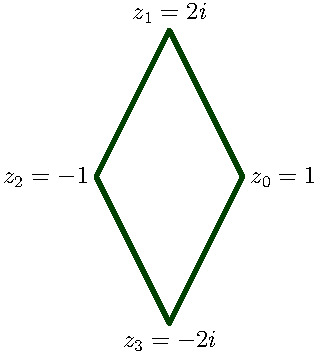
\includegraphics{./Eisoperi_1.pdf}
 % Eisoperi_1.pdf: 170x3 pixel, 72dpi, 6.00x0.11 cm, bb=0 0 170 3
 \caption{Un polygone à 4 côtés}
 \label{fig:Eisoperi_1}
\end{figure}

\subsection*{Partie I. Calculs préliminaires.}
\begin{enumerate}
 \item 
\begin{enumerate}
 \item Soit $k\in \llbracket 1 , n-1 \rrbracket$ et $\varepsilon\in\{-1,+1\}$. Montrer que 
\begin{displaymath}
 \sin\left( \frac{k\pi}{n}\right) +\varepsilon \tan\left( \frac{\pi}{n}\right) \cos\left( \frac{k\pi}{n}\right)\geq 0  
\end{displaymath}
\item En utilisant le tableau de variations de $x \rightarrow \tan x -x$ dans un intervalle à préciser, montrer que 
\begin{displaymath}
 n \tan\left( \frac{\pi}{n}\right) \geq \pi
\end{displaymath}

\end{enumerate}

\item Soit $Z=(z_0,\cdots,z_{n-1})$ un polygone régulier avec $a$ et $b$ comme dans la définition.
\begin{enumerate}
  \item Montrer que $Z$ est équilatéral.
  \item Montrer les points dont les affixes sont les $z_i$ sont sur un cercle dont on précisera le centre et le rayon.
  \item Exprimer $b$ puis $a$ en fonction des $z_i$.
\end{enumerate}
\item Montrer que le polygone de l'exemple de la figure \ref{fig:Eisoperi_1} est équilatéral mais pas régulier.
\item Soit $p\in \Z$, discuter selon $p$ de la valeur de 
\begin{displaymath}
 \frac{1}{\sqrt{n}}\sum_{k=0}^{n-1}(\omega^p)^k
\end{displaymath}
\item Soit $Z= (z_0,z_1,\cdots,z_{n-1})\in \C^n$. Vérifier que
\begin{displaymath}
 \forall j\in \{0,\cdots,n-1\},\; z_j = \frac{1}{\sqrt{n}}\sum_{k=0}^{n-1}(\omega^j)^k \widehat{z}_k 
\end{displaymath}
\end{enumerate}
\subsection*{Partie II. Inégalité isopérimétrique pour les polygones.}
Pour tout polygone $Z=(z_0,\cdots,z_{n-1})$, on définit $L(Z)$, $E(Z)$ et $A(Z)$ par:
\begin{displaymath}
 L(Z) = \sum_{k=0}^{n-1}|z_{k+1}-z_k|, \hspace{0.3cm}
 E(Z) = \sum_{k=0}^{n-1}|z_{k+1}-z_k|^2, \hspace{0.3cm}
 A(Z) = \frac{1}{2}\Im\left( \sum_{k=0}^{n-1}z_{k+1}\overline{z_k}\right) 
\end{displaymath}
Il est évident que $L(Z)$ est le périmètre du polygone. Le réel $A(Z)$ représente son \emph{aire algébrique} mais vous ne devez ni justifier ni utiliser cette propriété.
\begin{enumerate}
 \item Soit $c\in \C$ et $Z\in \C^n$. Exprimer $A(\overline{Z})$ et $A(Z+c)$ en fonction de $A(Z)$.
\item On suppose dans cette question seulement que $Z$ est un polygone régulier.
\begin{enumerate}
 \item Exprimer $L(Z)$, $E(Z)$, $A(Z)$ en fonction de $\sin\left( \frac{\pi}{n}\right)$ ou de $\sin\left( \frac{2\pi}{n}\right)$  
 \item En déduire les rapports
\begin{align*}
 \frac{|A(Z)|}{L(Z)^2} & & \frac{|A(Z)|}{E(Z)} & & \frac{L(Z)^2}{E(Z)} 
\end{align*}
\end{enumerate}
 
 \item Soit $Z\in \C^n$. Montrer que $L(Z)^2 \leq nE(Z)$. Sous quelle condition sur $Z$ a-t-on l'égalité?
 \item Soit $Z\in \C^n$.
\begin{enumerate}
 \item \'Etablir les relations
\begin{align*}
 A(Z) = \frac{1}{2}\sum_{k=0}^{n-1}\sin\left( \frac{2k\pi}{n}\right)|\widehat{z}_k|^2 & & 
 E(Z) = 4\sum_{k=0}^{n-1}\sin^2\left( \frac{k\pi}{n}\right)|\widehat{z}_k|^2
\end{align*}
\item Montrer que 
\begin{displaymath}
 E(Z) - 4 \tan\left( \frac{\pi}{n}\right)A(Z)
=
4 \sum_{k=0}^{n-1}\sin\left( \frac{k\pi}{n}\right)
\left[
\sin\left( \frac{k\pi}{n}\right) - \tan\left( \frac{\pi}{n}\right)\cos\left( \frac{k\pi}{n}\right)
 \right]
|\widehat{z}_k|^2
\end{displaymath}
\item Montrer que 
\begin{displaymath}
\frac{|A(Z)|}{E(Z)}\leq \frac{1}{4\tan\left( \frac{\pi}{n}\right) } 
\end{displaymath}
\end{enumerate}

\item On admet qu'il existe $Z_0\in \C^n$ tel que :
\begin{displaymath}
 \forall Z\in \C^n:\hspace{0.3cm}
\frac{|A(Z)|}{L(Z)^2} \leq \frac{|A(Z_0)|}{L(Z_0)^2}
\end{displaymath}
\begin{enumerate}
 \item Soit $(z_0, \cdots, z_{n-1})=Z_0$ et $j$ entier entre $0$ et $n-1$. On note $Z_1$ le polygone obtenu à partir de $Z$ en remplaçant $z_j$ par $z_j + \lambda(z_{j+1}-z_{j-1})$ (avec un $\lambda$ réel) sans changer les autres valeurs. Montrer que $A(Z_1)=A(Z_0)$.
 \item Montrer que $Z_0$ est équilatéral.
 \item Montrer l'inégalité isopérimétrique pour les polygones:
\begin{displaymath}
 \forall Z\in \C^n,\hspace{0.5cm} 4\pi |A(Z)|\leq L(Z)^2
\end{displaymath}
Ce qui prouve l'inégalité demandée pour le cas des polygones. Cette inégalité se généralise à d'autres courbes.
\end{enumerate}

\end{enumerate}
